\section{Architecture and API}
\begin{figure}[t]
% \vspace{-5pt}
\centering
 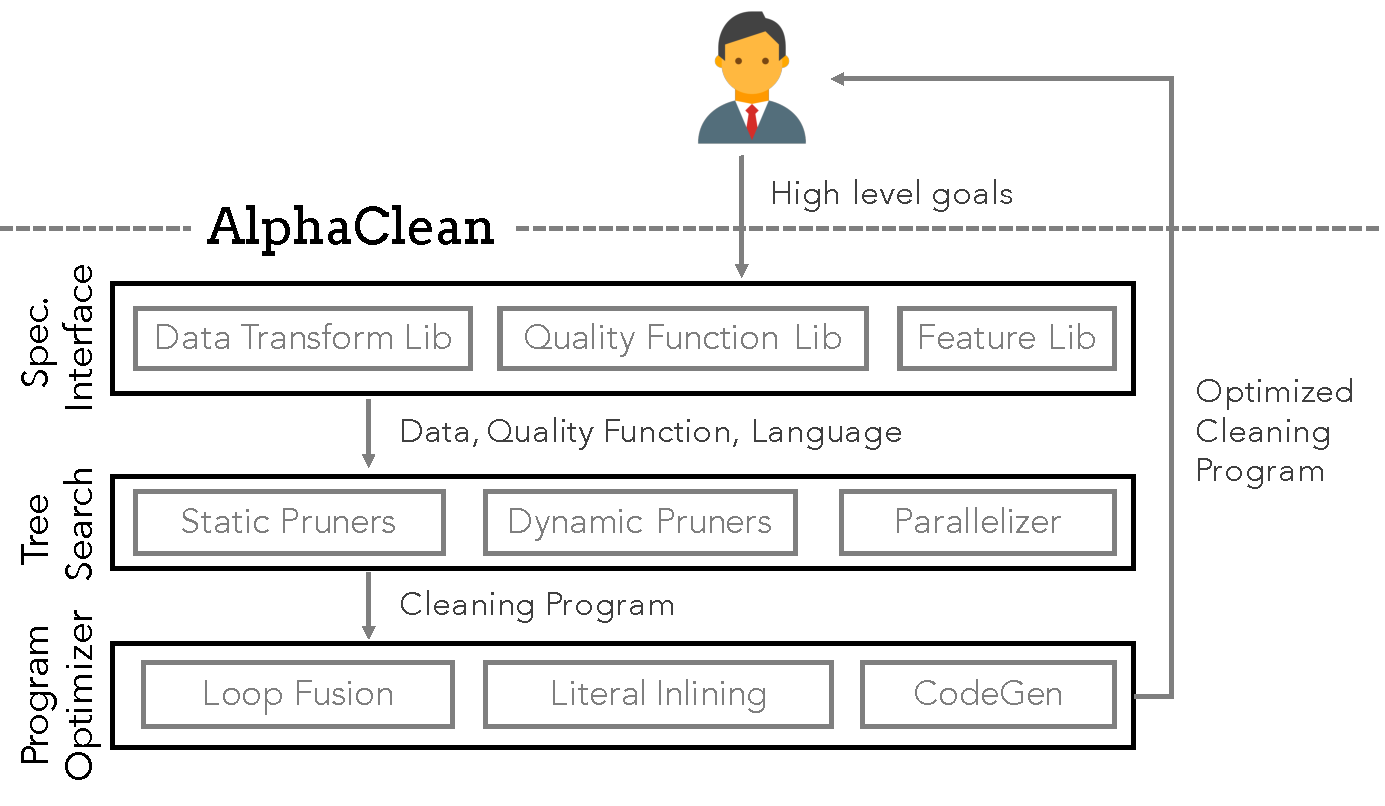
\includegraphics[width=\columnwidth]{figures/alphacleanarch.pdf}
 \caption{\small \sys transforms high level cleaning goals (e.g., integrity constraints, statistical models, cleaning operations) into a quality measure and cleaning language, and uses an optimized tree search to find and optimize a sequence of transformations (cleaning program) to maximize the quality measure.   \label{fig:arch} }
\end{figure}
This section describes the three major components of the \sys system architecture (\Cref{fig:arch}), split between the user interface to specify the cleaning problem, the core search algorithm, and optimization of the resulting cleaning program.  We detail the interface and program optimization in this section, and focus on the search algorithm and optimizations in the rest of the paper. Designing data cleaning interfaces~\cite{DBLP:conf/uist/GuoKHH11} and query optimization for data cleaning~\cite{DBLP:conf/vldb/GalhardasFSSS01, khayyat2015bigdansing} are interesting problems in their own right, and we believe \sys can enable simpler and more powerful approaches.  However, these were not a focus of the current study.

The {\it Specification Interface} contains extensible libraries of domain-specific quality functions, cleaning data transformations, and pruning feature hints that the user can use to define a high level cleaning goal.  Our current implementation can translate a wide range of domain-specific goals---including type constraints, functional dependencies, denial constraints, lookup tables, parametric and non-parametric outlier models, and correlations between numeric attributes---into a single quality function.  Users can also constrain the cleaning language, and we currently support any type of conditional cell and record transformation that applies a black-box transformation to all cells or records satisfying a predicate; both the transformation parameters and the predicate are learned by \sys.  Finally, users can optionally provide features that \sys uses to dynamically learn pruning rules (Section~\ref{s:dynlearn}).    \Cref{s:appendix} provides a detailed description of the supported functions and extensible API. 

The {\it Search} component takes as input the quality function $Q$ and language $L$, and performs a greedy search heuristic to find a program $p^* \in L$ that maximizes $Q$.  Users can supply hints that exploit the problem structure to reduce the runtime by pruning the search space and parallelizing the search.  To bound the search space, users specify a maximum program length $k$.    \sys also supports three classes optimizations. {\it Static pruning} invalidates candidate programs based on the program structure (sequence of actions).  For instance, composing the same idempotent transformation (e.g., \texttt{find\_replace(SFO, SF, city\_name)}) in succession is unnecessary.  {\it Dynamic pruning} can access the result of a candidate program (search state) when making pruning decisions, and we propose a novel approach to learn automatic dynamic pruning rules that can reduce end-to-end runtimes by up to 75\% at the expense of slightly lower recall. Finally, \sys {\it parallelizes} the search in both shared memory and distributed settings.   \Cref{s:search} describes the pruning rules and parallelization optimization in detail.


Finally, once search component outputs the cleaning program $p^*$, the {\it Program Optimizer} performs query compilation optimizations and provides an API to add new optimizations.  \sys currently replaces variables with literal values whenever possible, inlines data transformations into loops that scan over the input relation, and uses loop fusion~\cite{palkar2017weld, crotty2014tupleware} to avoid unnecessary scans over the input and intermediate relations for each transformation in $p^*$.  Consider the program in~\Cref{ex3}.  Since the \texttt{find\_replace} operations do not conflict, it is inefficient to loop through over the relation instance three separate times.  Since they do not conflict, it would be inefficient to execute them sequentially and iterate over the data three separate times.  Instead, they can be fused:
{\small
\begin{lstlisting}
    for r in rows:
     if r[city_name] == `New York':
       r[city_name] = `New York City'
     elif r[city_name] == `San Francisc':
       r[city_name] = `San Francisco'
     if r[city_code] == `NYC'
       r[city_code] = `NY'
\end{lstlisting}
}
These simple optimizations improve the final program runtime by up-to 20x, and we leave further improvements to future work (e.g., could be optimized with a framework like Weld~\cite{palkar2017weld}).


% The user can optionally provide custom quality functions and data transformations as simple Python class definitions.      takes as input user specifications of the quality function and data transformation language, alongside search configuration parameters.


\if{0}
Now, we will overview some of the preliminary concepts and describe how this formalism inspires a modular system API.
\sys is designed as a software stack with three layers: a specification layer, a search layer, and an execution layer.
To understand how these layers interact, we will use the example in Section 2 throughout this section.


\subsection{Specification Layer} The provides an API for specifying a quality function and a language of transformations. This allows one to specify a data cleaning problem for a particular dirty instance. As described in the previous section, we provide an API for translating common data cleaning specifications, constraints, statistical models, and gold standard examples, into quality functions. 

The harder problem is specifying the language. 
The challenge is that most data transformations are parametrized by literal values from the database.
We need efficient techniques to automatically enumerate this transformation set before we apply the search.
The language is generated through a transformation templates which are dynamically populated by literals in the database.
A template is a parametrized transformation:
\[T(R, [\theta_1, \theta_2,...,\theta_k] ): \mathcal{R} \mapsto  \mathcal{R},\] where the parameters $[\theta_i]$ are populated by literal values.
Each $\theta_i$ represents an SQL query except for special parameters such as attribute names and data-independent hyperparameters.
The system dynamically generates all possible literal instances of this transformation by taking the cartesian product of the query results.

In the running example, consider the following function:
\[
\textsf{find\_replace}(\text{source}, \text{target}, \text{attribute})
\]
\begin{lstlisting}
source := SELECT attribute from R;
target := SELECT attribute from R;
\end{lstlisting}
Likewise for numerical transformations, consider the function that clips outlier values outside 6 standard deviations of the mean:
\[
\textsf{clip}(\text{mean}, \text{threshold})
\]
\begin{lstlisting}
mean := SELECT mean(attribute) from R;
threshold := SELECT 6*std(attribute) from R;
\end{lstlisting}
\sys provides queries and filters for a number of common parametrizations or they can be specified manually.

\subsection{Search Layer (Section 5)} The next layer is the search layer, which implements the basic search algorithm of \sys. This algorithm is a distributed best-first greedy search.  
With no additional information, the search approach described would have to evaluate $61^3 = 226981$ transformations, which is clearly impractical even for this small example.
This layer also provides an interface for custom search optimizations:

\fi
